\documentclass[11pt,a4paper]{article}
\usepackage[margin=24mm]{geometry}
\usepackage{amsmath,amssymb,amsthm,bm}
\usepackage{graphicx}
\usepackage{booktabs}
\usepackage{xcolor}
\usepackage{tikz}
\usetikzlibrary{arrows.meta,positioning}
\usepackage[hidelinks]{hyperref}
\usepackage{caption}
\usepackage{enumitem}
\setlist{itemsep=2pt,topsep=4pt}
\captionsetup{font=small,labelfont=bf}
\graphicspath{{../}}
\definecolor{navy}{HTML}{1F3B63}
\newcommand{\E}{\mathbb{E}}
\newcommand{\R}{\mathbb{R}}
\newcommand{\C}{\mathbb{C}}
\newcommand{\Q}{\operatorname{Q}}
\newtheorem*{example}{Worked example}
\setlength{\parskip}{4pt}
\setlength{\parindent}{0pt}

\title{\color{navy}\textbf{Sending Pictures With Sound}\\[4pt]\large The theory behind an acoustic OFDM link}
\author{acoustic\_ofdm\_matlab}
\date{}

\begin{document}
\maketitle

\begin{abstract}
This document explains, from first principles, every block of the acoustic
link in this project: how a picture becomes bits, how bits become tones, why
OFDM turns an echoey room into many simple channels, how the receiver finds,
measures and undoes the room, how it detects and corrects errors, and what
the live results tell us about real speakers and microphones. Each section
gives the mathematics, the numbers used in the code, and a short worked
example. Notation is summarised in Appendix~\ref{app:notation}.
\end{abstract}

\tableofcontents
\newpage

%=====================================================================
\section{The problem and the system at a glance}
%=====================================================================

We want to move a $64\times64$ grayscale picture (4096 bytes) from one device
to another using only a loudspeaker and a microphone. Sound in a room is a
\emph{wideband, frequency-selective, noisy, slightly time-varying} channel:
walls create echoes, transducers favour some frequencies over others, the two
devices run on independent clocks, and operating systems sometimes process
audio in ways no textbook channel model includes.

The design answers each of these with a standard communications tool:

\begin{center}
\begin{tabular}{@{}ll@{}}
\toprule
Impairment & Answer in this project \\
\midrule
Echoes (multipath) & OFDM with a cyclic prefix \\
Uneven frequency response & Training symbols and one-tap equalisation \\
Unknown start time & Chirp preamble and matched filtering \\
Clock mismatch & Pilot tones and phase-slope tracking \\
Residual bit errors & CRC32 detection, optional convolutional coding \\
\bottomrule
\end{tabular}
\end{center}

\begin{figure}[h]
\centering
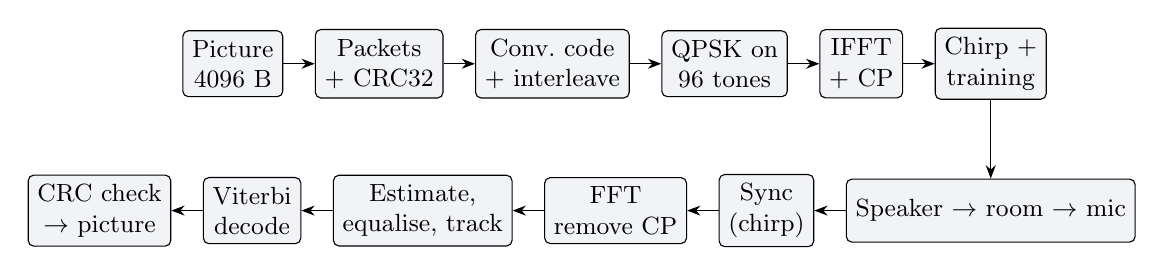
\begin{tikzpicture}[node distance=4mm and 4mm, >=Stealth,
  box/.style={draw, rounded corners=2pt, fill=navy!6, minimum height=8mm, align=center, font=\small}]
\node[box] (img) {Picture\\4096 B};
\node[box, right=of img] (pkt) {Packets\\+ CRC32};
\node[box, right=of pkt] (fec) {Conv.\ code\\+ interleave};
\node[box, right=of fec] (map) {QPSK on\\96 tones};
\node[box, right=of map] (ofdm) {IFFT\\+ CP};
\node[box, right=of ofdm] (frame) {Chirp +\\training};
\node[box, below=10mm of frame] (spk) {Speaker $\to$ room $\to$ mic};
\node[box, left=of spk] (sync) {Sync\\(chirp)};
\node[box, left=of sync] (fft) {FFT\\remove CP};
\node[box, left=of fft] (eq) {Estimate,\\equalise, track};
\node[box, left=of eq] (dec) {Viterbi\\decode};
\node[box, left=of dec] (crc) {CRC check\\$\to$ picture};
\draw[->] (img)--(pkt); \draw[->] (pkt)--(fec); \draw[->] (fec)--(map);
\draw[->] (map)--(ofdm); \draw[->] (ofdm)--(frame); \draw[->] (frame)--(spk);
\draw[->] (spk)--(sync); \draw[->] (sync)--(fft); \draw[->] (fft)--(eq);
\draw[->] (eq)--(dec); \draw[->] (dec)--(crc);
\end{tikzpicture}
\caption{Transmit chain (top, left to right) and receive chain (bottom, right to left).
The coding block is optional (the \texttt{'fec'} flag).}
\end{figure}

%=====================================================================
\section{Sound as a communication channel}
%=====================================================================

\subsection{Discrete-time model}
Everything is sampled at $f_s=48\,$kHz. The transmitted waveform $x[n]$ is
real. Played through a speaker, shaped by the room and captured by a
microphone, it arrives as
\begin{equation}
y[n] = \sum_{\ell=0}^{L-1} h[\ell]\,x[n-\ell] + w[n],
\label{eq:lti}
\end{equation}
where $h[\ell]$ is the combined impulse response of speaker, room and
microphone and $w[n]$ is additive noise. Equation~\eqref{eq:lti} assumes the
path is \emph{linear} and \emph{time-invariant} (LTI) over a packet. It is a
good model for a phone or a laptop with audio effects switched off, and a poor
one when the operating system compresses or re-equalises the sound
(Section~\ref{sec:windows}).

\subsection{Frequency selectivity}
In the frequency domain the channel multiplies each frequency by
$H(f)=\sum_\ell h[\ell]e^{-j2\pi f\ell/f_s}$. A direct path plus one echo of
relative amplitude $a$ and delay $\tau$ gives
\[
|H(f)|^2 = 1 + a^2 + 2a\cos(2\pi f\tau),
\]
which has notches every $1/\tau$ hertz. An echo 2\,ms late notches the
spectrum every 500\,Hz. With many echoes the response becomes the jagged
curve seen in our measurements, with dips of 10--20\,dB at some frequencies
(for example near 4 and 6.5\,kHz in the phone runs).

\subsection{Delay spread and coherence bandwidth}
Treat $p_\ell=|h[\ell]|^2/\sum|h|^2$ as a distribution over delay
$\tau_\ell=\ell/f_s$. Its mean and RMS width are
\[
\bar\tau=\sum_\ell p_\ell\tau_\ell,\qquad
\tau_{\mathrm{rms}}=\sqrt{\textstyle\sum_\ell p_\ell(\tau_\ell-\bar\tau)^2}.
\]
Frequencies closer together than the \emph{coherence bandwidth}
$B_c\approx 1/(5\tau_{\mathrm{rms}})$ see roughly the same gain. This number
tells us how far apart pilot tones may be and how far apart the interleaver
must spread neighbouring coded bits.

\subsection{Reverberation}
A room's late reverberation decays roughly exponentially. The reverberation
time $\mathrm{RT}_{60}$ is the time for energy to fall by 60\,dB, so the
amplitude envelope is $\exp(-3\ln 10\, t/\mathrm{RT}_{60})$. The
direct-to-reverberant ratio (DRR) compares the energy of the direct sound to
everything after it. Close to the speaker the DRR is high and the room
barely matters; a few metres away the reverberant tail dominates. Our stress
test models a room exactly this way: a unit direct path plus a Gaussian tail
with the chosen $\mathrm{RT}_{60}$ and DRR.

%=====================================================================
\section{OFDM from first principles}
%=====================================================================

\subsection{Many slow carriers instead of one fast one}
A single-carrier signal at a few kilobits per second would have symbols much
shorter than the room's echoes, so every symbol would smear into the next
(inter-symbol interference, ISI) and the receiver would need a long adaptive
equaliser. OFDM instead splits the band into $K$ narrow subcarriers, each
carrying a slow stream of symbols. Each symbol lasts $N/f_s=21.3\,$ms, far
longer than most short-range echoes, and each narrow subcarrier sees an
almost flat channel: a single complex gain.

\subsection{Orthogonality and the DFT}
Let $N=1024$. The complex exponentials
$\phi_k[n]=e^{j2\pi kn/N}$, $n=0,\dots,N-1$, satisfy
\begin{equation}
\sum_{n=0}^{N-1}\phi_k[n]\,\phi_m^*[n] = N\,\delta_{km},
\end{equation}
so they are orthogonal over one symbol: tones on different bins can overlap
in frequency without interfering, provided the receiver looks at exactly $N$
samples. The subcarrier spacing is $\Delta f=f_s/N=46.875\,$Hz.

Placing complex symbols $X_k$ on the bins and summing gives the transmitted
symbol, which is exactly an inverse DFT. The code uses the \emph{unitary}
pair
\begin{equation}
x[n] = \frac{1}{\sqrt N}\sum_{k=0}^{N-1}X_k e^{j2\pi kn/N},
\qquad
X_k = \frac{1}{\sqrt N}\sum_{n=0}^{N-1}x[n]e^{-j2\pi kn/N},
\end{equation}
implemented as \texttt{sqrt(N)*ifft(X)} and \texttt{fft(x)/sqrt(N)}. With this
scaling Parseval's theorem reads $\sum_n|x[n]|^2=\sum_k|X_k|^2$, so energy per
symbol is the same in both domains and SNR can be quoted per subcarrier
without extra factors.

\subsection{A real-valued waveform: Hermitian symmetry}
A speaker needs a real signal. A sequence is real exactly when its DFT is
conjugate-symmetric, $X_{N-k}=X_k^*$. We therefore load data on the
\emph{positive} bins $k=43,\dots,170$ and put their complex conjugates on bins
$N-k$. The IFFT output is then real (the code asserts the imaginary part is
below $10^{-12}$). The mirror doubles the transmitted energy but carries no
new information.

\begin{example}
Bins 43 to 170 at $\Delta f=46.875\,$Hz cover $2015.6$ to $7968.8\,$Hz: 128
subcarriers inside the 2--8\,kHz band, where phone and laptop speakers are
reasonably efficient and room noise (fans, hum, voices) is low.
\end{example}

\subsection{The cyclic prefix}
\label{sec:cp}
Before sending each symbol we copy its last $N_{\mathrm{cp}}=256$ samples
($5.33\,$ms) to its front. If the channel is shorter than the prefix,
$L\le N_{\mathrm{cp}}+1$, then inside the receiver's $N$-sample window the
linear convolution \eqref{eq:lti} is indistinguishable from a
\emph{circular} convolution. The DFT turns circular convolution into
multiplication, so for every used bin
\begin{equation}
\boxed{\,Y_k = H_k X_k + W_k\,}
\label{eq:perbin}
\end{equation}
with $H_k=\sum_\ell h[\ell]e^{-j2\pi k\ell/N}$ and $W_k$ the noise. The whole
room collapses to one complex number per subcarrier. This is the central
reason OFDM works.

\emph{Proof sketch.} Write the received window as
$y[n]=\sum_\ell h[\ell]\tilde x[n-\ell]+w[n]$ for $n=0..N-1$, where $\tilde x$
is the prefixed symbol. For $\ell\le N_{\mathrm{cp}}$ the index $n-\ell$ falls
either in the symbol or in its prefix, and the prefix equals the symbol's
tail, so $\tilde x[n-\ell]=x[(n-\ell)\bmod N]$: a circular shift. Taking the
DFT of a circular convolution gives \eqref{eq:perbin}.

\textbf{When the prefix is too short.} Energy arriving later than
$N_{\mathrm{cp}}$ samples belongs to the \emph{previous} symbol (ISI) and
breaks the circular structure, leaking power between subcarriers
(inter-carrier interference, ICI). Neither can be removed by a one-tap
equaliser. If a fraction $\eta$ of the channel energy lies outside the
prefix, the best achievable signal-to-interference ratio is roughly
\[
\mathrm{SIR}\approx\frac{1-\eta}{\eta},
\]
which caps the effective SNR however loud the signal is. The receiver
reports $\eta$ as ``energy outside the cyclic prefix''. In the stress test,
the 2-metre room has $\eta\approx-4\,$dB, which caps the SNR near 4\,dB, and
no amount of power or coding helps. The single-laptop run had $-28\,$dB.

\textbf{Overhead.} The prefix costs $N_{\mathrm{cp}}/(N+N_{\mathrm{cp}})=20\%$
of air time. It is a deliberate trade: long enough for desk-scale echoes,
short enough not to waste most of the time.

\textbf{Timing tolerance.} Any FFT window start inside the prefix still sees
a circular convolution, only with an extra linear phase (a pure delay). The
receiver therefore starts its window 32 samples \emph{before} the estimated
strongest arrival, so slightly early paths and timing jitter stay inside the
prefix.

%=====================================================================
\section{Modulation: putting bits on a tone}
%=====================================================================

\subsection{QPSK with Gray mapping}
Each data subcarrier carries two bits $(b_1,b_2)$ as
\begin{equation}
X = \frac{(1-2b_1) + j(1-2b_2)}{\sqrt2},
\end{equation}
so $|X|^2=E_s=1$. The bits are independent on the two axes, which is a Gray
mapping: neighbouring points differ in one bit. The receiver decides
$\hat b_1=[\Re\{\hat X\}<0]$, $\hat b_2=[\Im\{\hat X\}<0]$.

\subsection{Error probability}
After equalisation (Section~\ref{sec:eq}) a subcarrier sees
$\hat X=X+V$ with complex Gaussian noise of variance $\sigma^2$, i.e.\
$\sigma^2/2$ per axis. Define the per-subcarrier SNR $\gamma=E_s/\sigma^2$.
Bit $b_1$ is wrong when the real-axis noise exceeds $1/\sqrt2$:
\begin{equation}
P_b^{\mathrm{QPSK}} = \Q\!\left(\frac{1/\sqrt2}{\sqrt{\sigma^2/2}}\right)
=\Q\!\left(\sqrt{\gamma}\right),\qquad
\Q(x)=\frac{1}{\sqrt{2\pi}}\int_x^\infty e^{-t^2/2}\,dt.
\end{equation}
For comparison $P_b^{\mathrm{BPSK}}=\Q(\sqrt{2\gamma})$, and Gray 16-QAM has
$P_b=\tfrac34\Q(a)+\tfrac12\Q(3a)-\tfrac14\Q(5a)$ with $a=\sqrt{\gamma/5}$.
QPSK needs $\gamma\approx9.8\,$dB for $P_b=10^{-3}$. Our Monte Carlo
simulations agree with all three formulas (Figure~\ref{fig:awgn}).

\begin{figure}[h]
\centering
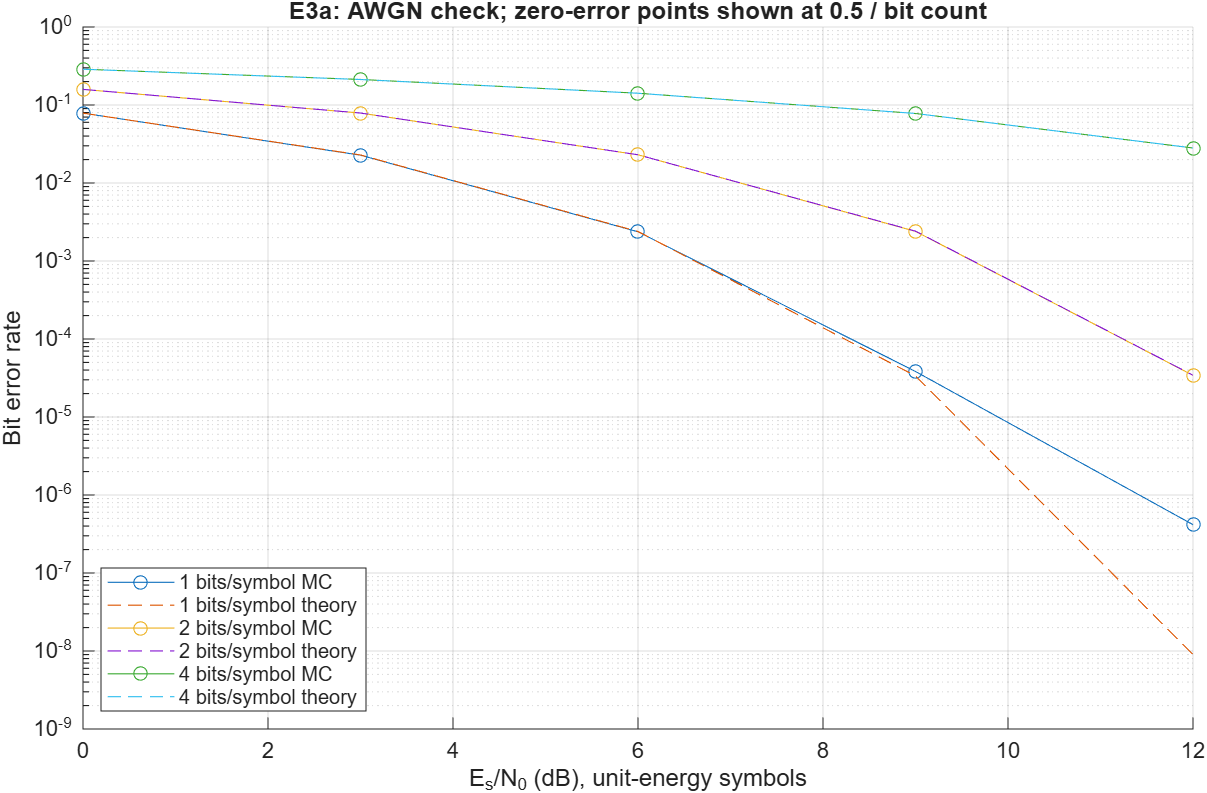
\includegraphics[width=0.72\linewidth]{figures/E3a_awgn.png}
\caption{Simulated bit error rate (circles) against theory (dashed) for
BPSK, QPSK and 16-QAM in white Gaussian noise.}
\label{fig:awgn}
\end{figure}

\subsection{Error vector magnitude}
The receiver also reports the EVM, the average squared distance from each
equalised symbol to its nearest constellation point:
$\mathrm{EVM}=\E|\hat X-\mathrm{dec}(\hat X)|^2$. At moderate SNR this is
close to $1/\gamma$, so $\mathrm{EVM}_{\mathrm{dB}}\approx-\gamma_{\mathrm{dB}}$.
EVM is measured on the data, while the receiver's SNR estimate comes from the
training symbols. A large gap between the two, such as SNR 10\,dB but EVM
$-3\,$dB, means the data saw something the training did not: a channel that
changed during the packet, or distortion.

%=====================================================================
\section{Packet and frame design}
%=====================================================================

\subsection{From picture to packets}
The 4096 picture bytes are split into 64 packets. Each packet is
\[
\underbrace{\text{ID}_{\text{hi}},\text{ID}_{\text{lo}},\text{len}_{\text{hi}},\text{len}_{\text{lo}}}_{4\text{ B header}}
\;\big|\;\underbrace{64\text{ image bytes}}_{\text{one column of pixels}}
\;\big|\;\underbrace{\text{CRC32}}_{4\text{ B}}
\;=\;72\text{ B}=576\text{ bits}.
\]
MATLAB stores images column by column, so a lost packet leaves one gray
\emph{column}, which is the thin vertical line in the received pictures.

\subsection{Carrier layout}
Of the 128 used subcarriers, every fourth (32 in total) is a \emph{pilot}
with a known value, and the other 96 carry data. One OFDM symbol therefore
carries $96\times2=192$ bits. The raw rate is
\[
\frac{192\text{ bits}}{(1024+256)/48000\text{ s}} = 7200\text{ bit/s},
\]
before the preamble, training, gaps and checksum are paid for.

\subsection{One packet on air}
\begin{center}
\begin{tabular}{@{}lrr@{}}
\toprule
Part & Samples & Duration \\
\midrule
Chirp preamble (1$\to$9\,kHz, Hann-tapered) & 2400 & 50\,ms \\
Guard silence & 1440 & 30\,ms \\
Two identical training symbols & $2\times1280$ & 53\,ms \\
Data symbols, uncoded: 3 & $3\times1280$ & 80\,ms \\
Data symbols, coded: 7 & $7\times1280$ & 187\,ms \\
Gap before next packet & 1440 & 30\,ms \\
\bottomrule
\end{tabular}
\end{center}
Uncoded, a packet is 11{,}680 samples, the picture takes 16.0\,s and the net
rate is $32768/16.02\approx2045\,$bit/s. With coding, a packet is 16{,}800
samples, the picture takes 22.9\,s and the rate is about 1430\,bit/s.

%=====================================================================
\section{Synchronisation: finding the packet}
%=====================================================================

\subsection{Why a chirp}
The preamble is a linear frequency sweep,
\[
c(t)=w(t)\sin\!\Big(2\pi\big(f_0t+\tfrac{f_1-f_0}{2T}t^2\big)\Big),\qquad
f_0=1\,\text{kHz},\; f_1=9\,\text{kHz},\; T=50\,\text{ms},
\]
with a Hann window $w(t)$ to soften its edges. A chirp is easy to detect even
when the room colours it: its energy is spread over the whole band, so a
notch at one frequency only removes a small part of it, and its
autocorrelation is a sharp peak. The time-bandwidth product
$BT=8000\times0.05=400$ gives a processing gain of about
$10\log_{10}400\approx26\,$dB and a timing resolution of order
$1/B\approx0.13\,$ms.

\subsection{Normalised matched filter}
The receiver slides the known chirp $c$ along the recording and computes
\begin{equation}
\rho[m]=\frac{\big|\sum_{i}y[m+i]\,c[i]\big|}
{\sqrt{\sum_i y[m+i]^2\;\sum_i c[i]^2}}\in[0,1],
\end{equation}
which by the Cauchy--Schwarz inequality equals 1 only for a perfect match
and does not depend on volume. It takes the \emph{first} index where
$\rho$ exceeds $\max(0.12,\;0.65\max\rho)$ and then the local maximum just
after it. Choosing the first strong peak, rather than the global one,
prevents locking onto a late echo of the chirp. The correlation is computed
with FFTs, so scanning a 45-second recording is fast.

\subsection{Fine timing}
The chirp gives a coarse position. The receiver then correlates against the
known training symbol within $\pm N_{\mathrm{cp}}$ samples of where it should
be, takes the strongest match, and backs off 32 samples into the cyclic
prefix (Section~\ref{sec:cp}). After a packet is decoded the search for the
next chirp starts just after it, so every packet resynchronises on its own.
A missed or late start costs packets but does not shift later ones.

%=====================================================================
\section{Estimating the channel}
%=====================================================================

\subsection{Least squares from training symbols}
Each packet starts with two identical OFDM symbols carrying known QPSK values
$S_k$ on all 128 used bins. From \eqref{eq:perbin}, $Y_k^{(i)}=H_kS_k+W_k^{(i)}$,
so the least-squares estimate averages the two:
\begin{equation}
\hat H_k=\frac{Y_k^{(1)}+Y_k^{(2)}}{2S_k}=H_k+\frac{W_k^{(1)}+W_k^{(2)}}{2S_k}.
\end{equation}
Averaging halves the noise variance in the estimate. $\hat H_k$ automatically
includes the transmit gain, the speaker and microphone sensitivity and the
room, which is why the absolute playback volume never needs to be known.

\subsection{Measuring the noise for free}
Subtracting the two training symbols cancels the channel:
$Y_k^{(1)}-Y_k^{(2)}=W_k^{(1)}-W_k^{(2)}$, and for independent noise
\begin{equation}
\E\,|Y_k^{(1)}-Y_k^{(2)}|^2=2\sigma_k^2
\quad\Longrightarrow\quad
\hat\sigma_k^2=\tfrac12|Y_k^{(1)}-Y_k^{(2)}|^2,
\end{equation}
smoothed over 9 neighbouring bins to reduce its variance. The per-bin SNR
reported everywhere in this project is
\[
\hat\gamma_k=\frac{|\hat H_k|^2E_s}{\hat\sigma_k^2}.
\]
This estimate sees additive noise and anything else that differs between the
two training symbols. It does \emph{not} see distortion that affects both
equally, nor changes that happen later in the packet. That is why EVM is
reported as well.

\subsection{L-MMSE estimation (simulation study)}
In the simulation study the channel is learned from comb pilots only, and we
compare least squares (LS) with linear minimum mean-square error (L-MMSE)
estimation. Stack the pilot observations $\bm z=\bm Y_p/\bm X_p=\bm H_p+\bm v$.
We seek the linear estimator $\hat{\bm H}=\bm W\bm z$ minimising
$\E\|\bm H-\bm W\bm z\|^2$. The orthogonality principle requires the error
to be uncorrelated with the data:
\[
\E\big[(\bm H-\bm W\bm z)\bm z^H\big]=\bm 0
\;\Rightarrow\;
\bm W=\bm R_{H\!p}\,\big(\bm R_{pp}+\bm C_v\big)^{-1},
\]
where $\bm R=\E[\bm H\bm H^H]$ is the channel's frequency correlation,
computed from its delay profile $\bm p$ as
\[
\bm R=\bm F\,\mathrm{diag}(\bm p)\,\bm F^H,
\]
$\bm R_{H\!p}$ holds its columns at the pilots, $\bm R_{pp}$ is the pilot
block and $\bm C_v$ the pilot noise covariance. The error covariance is
\begin{equation}
\bm C_e=\bm R-\bm W\bm R_{pH}.
\end{equation}
L-MMSE uses the correlation between neighbouring carriers to denoise and
interpolate at the same time. In the scalar case with prior variance 1 and
pilot noise 0.25, $W=1/1.25=0.8$ and the error variance falls from 0.25 (LS)
to 0.2.

\begin{figure}[h]
\centering
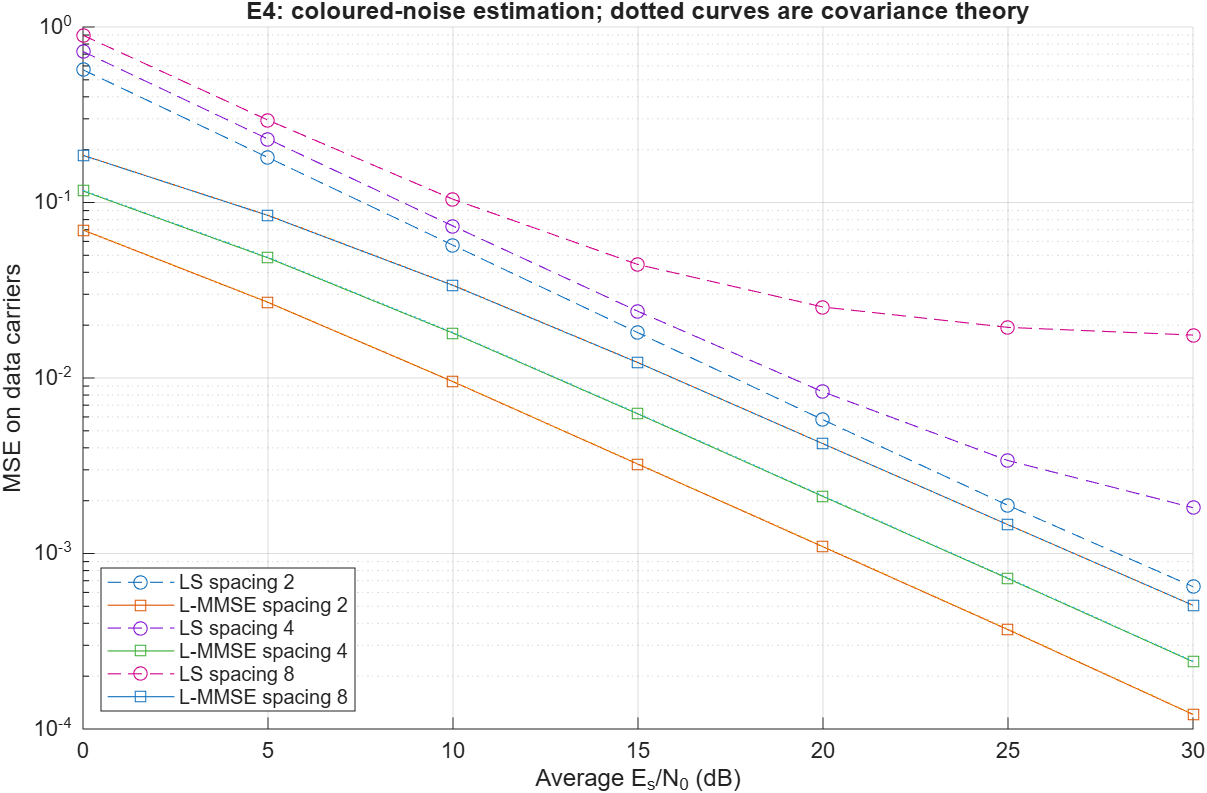
\includegraphics[width=0.72\linewidth]{figures/E4_estimation.png}
\caption{Channel-estimation error on data carriers. L-MMSE (squares) beats
LS (circles) at every pilot spacing; with sparse pilots LS interpolation hits
an error floor. Simulated MSE matches the covariance theory to within 1\%.}
\end{figure}

%=====================================================================
\section{Equalisation and clock tracking}
%=====================================================================

\subsection{One-tap equalisation}
\label{sec:eq}
Given $\hat H_k$, each data subcarrier is equalised by a single division,
\begin{equation}
\hat X_k=\frac{Y_k}{\hat H_k}=X_k+\frac{W_k}{\hat H_k}+\text{(estimation error)}.
\end{equation}
This is the zero-forcing equaliser. Its weakness is \emph{noise enhancement}:
on a subcarrier in a deep notch $|\hat H_k|$ is small and the noise is
divided by a small number. That subcarrier's bits are unreliable, which is
exactly the information the soft decoder in Section~\ref{sec:fec} uses.

\subsection{Why the phase drifts}
The two devices' sample clocks differ by $\varepsilon$ (typically tens of parts
per million). After $n$ samples the receiver's timing has slipped by
$d\approx\varepsilon n$ samples. A delay of $d$ samples multiplies bin $k$ by
$e^{-j2\pi kd/N}$, so the phase error grows \emph{linearly with frequency}
and \emph{linearly with time}.

\begin{example}
At $\varepsilon=20\,$ppm, a 0.35-second coded packet slips
$0.35\times48000\times20\times10^{-6}\approx0.34$ samples. At bin 170 that is
a phase error of $2\pi\cdot170\cdot0.34/1024\approx0.35\,$rad, about
20$^\circ$, enough to push QPSK points toward the decision boundaries if not
corrected.
\end{example}

\subsection{Pilot-based correction}
In every data symbol the receiver compares each pilot with its expected value
$\hat H_kP_k$, unwraps the phase differences $\theta_k$, and fits a straight
line $\theta_k\approx a+b(k-\bar k)$ by weighted least squares with weights
$|\hat H_k|$ (strong pilots count more). It then rotates every subcarrier by
$-(a+b(k-\bar k))$. The intercept $a$ absorbs common phase changes; the slope
$b$ absorbs timing drift. A unit test applies $a=0.3$, $b=0.002$ and removes
them to numerical precision, and a full packet survives a 30\,ppm resampling.
What this cannot fix is the small ICI caused by the drift itself, which is
negligible at these clock offsets.

%=====================================================================
\section{Detecting errors: CRC32}
%=====================================================================

\subsection{Polynomial arithmetic}
Treat the packet's bits as the coefficients of a polynomial $M(x)$ over
$\mathrm{GF}(2)$ (addition is XOR). The transmitter appends the remainder of
$x^{32}M(x)$ divided by the generator
\[
G(x)=x^{32}+x^{26}+x^{23}+x^{22}+x^{16}+x^{12}+x^{11}+x^{10}+x^{8}+x^{7}+x^{5}+x^{4}+x^{2}+x+1,
\]
so that the whole transmitted polynomial is divisible by $G(x)$ (the
standard CRC-32 also inverts the initial value and the result). The receiver
recomputes the CRC; any error pattern $E(x)$ that is not itself a multiple of
$G(x)$ is detected.

\subsection{What it guarantees}
For a 576-bit packet CRC-32 detects every error pattern of up to four bits,
every burst of up to 32 bits, and all but about $2^{-32}\approx2.3\times
10^{-10}$ of random patterns. It \emph{detects}; it cannot say which bit is
wrong. A packet is therefore accepted only if every bit is right.

\subsection{Bit errors versus packet errors}
If bits fail independently with probability $p$, a 576-bit packet survives
with probability
\begin{equation}
P_{\mathrm{pkt}}=(1-p)^{576}\approx e^{-576p}.
\end{equation}
\begin{center}
\begin{tabular}{@{}rr@{}}
\toprule
Bit error rate $p$ & Packets passing \\
\midrule
$1.2\times10^{-2}$ (our phone run, uncoded) & $0.09\%$ \\
$10^{-3}$ & $56\%$ \\
$2\times10^{-4}$ & $89\%$ \\
$10^{-5}$ & $99.4\%$ \\
\bottomrule
\end{tabular}
\end{center}
This ``cliff'' explains our most important live observation: a link where
98.8\% of bits arrive correctly still delivers essentially nothing.

%=====================================================================
\section{Correcting errors: convolutional coding}
\label{sec:fec}
%=====================================================================

\subsection{The encoder}
The encoder is a shift register holding the last six input bits. For every
input bit $u_t$ it outputs two coded bits, each the XOR of a fixed subset of
the register:
\[
c^{(1)}_t=\bigoplus_{i=0}^{6}g^{(1)}_i u_{t-i},\qquad
c^{(2)}_t=\bigoplus_{i=0}^{6}g^{(2)}_i u_{t-i},
\]
with generators $g^{(1)}=133_8=1011011_2$ and $g^{(2)}=171_8=1111001_2$.
This is the rate-$\tfrac12$, constraint-length-7 code used by IEEE 802.11
Wi-Fi. Six zero ``tail'' bits flush the register so the decoder knows the
final state. A 576-bit packet becomes $2(576+6)=1164$ coded bits, padded to
seven OFDM symbols (1344 bit slots).

\subsection{Why it can correct errors}
Every input bit influences 14 output bits (two outputs over seven steps), so
information is spread redundantly. The key number is the code's \emph{free
distance} $d_{\mathrm{free}}=10$: any two different coded sequences differ in
at least 10 bit positions. With soft decisions the asymptotic coding gain is
\[
G_c\approx10\log_{10}\!\big(R\,d_{\mathrm{free}}\big)=10\log_{10}5\approx7\,\text{dB},
\]
meaning the coded link needs roughly 7\,dB less SNR than the uncoded one for
the same error rate at high SNR. Our simulation agrees: at 4\,dB SNR,
40/40 coded packets passed against 2/40 uncoded.

\subsection{Soft information from QPSK}
Rather than hard 0/1 decisions, the decoder receives a log-likelihood ratio
for every coded bit. For bit $b_1$ on a subcarrier with equalised symbol
$\hat X$ and post-equalisation noise variance $\sigma^2/|\hat H|^2$,
\begin{equation}
\mathrm{LLR}(b_1)=\ln\frac{P(b_1=0\mid\hat X)}{P(b_1=1\mid\hat X)}
=\frac{2\sqrt2\,\Re\{\hat X\}\,|\hat H|^2}{\sigma^2}
\;\propto\;\Re\{\hat X\}\cdot\hat\gamma_k,
\end{equation}
and likewise $\Im\{\hat X\}$ for $b_2$. The sign is the hard decision; the
magnitude is the confidence, and it is \emph{weighted by that subcarrier's
SNR}. A bit from a tone in a 15\,dB notch therefore counts for about thirty
times less than a bit from a strong tone. The common factor $2\sqrt2$ does not
change the Viterbi decision, so the code uses $\Re\{\hat X\}\hat\gamma_k$.

\subsection{Interleaving}
Neighbouring subcarriers fade together (Section~2.3). If consecutive coded
bits sat on neighbouring tones, one notch would wipe out a run of them, and
convolutional codes handle runs poorly. A block interleaver writes the 1344
coded bits row by row into a $84\times16$ array and reads them column by
column. Consecutive coded bits end up 84 bit slots, i.e.\ 42 subcarriers or
about 2\,kHz, apart, so a notch produces isolated errors scattered through
the code sequence.

\subsection{The Viterbi algorithm}
The encoder is a finite-state machine with $2^6=64$ states. Each input bit
moves it along one of two branches, each labelled with two output bits. Given
LLRs $L^{(1)}_t,L^{(2)}_t$, the branch metric is
\[
\lambda_t(s\to s')=L^{(1)}_t\,(1-2c^{(1)})+L^{(2)}_t\,(1-2c^{(2)}),
\]
which is large when the branch's outputs agree with the confident received
values. The maximum-likelihood coded sequence maximises the sum of branch
metrics. Viterbi's insight is that only the best path into each state needs
to be kept:
\[
M_t(s')=\max_{s\to s'}\big[M_{t-1}(s)+\lambda_t(s\to s')\big].
\]
After the last (tail) bit the decoder starts from state 0 and traces the
stored decisions backwards. The cost is $64\times2$ additions per bit, so a
packet decodes in milliseconds.

The receiver also counts how many coded bits the decoder had to overrule
(re-encode the decoded bits, compare with the hard decisions). This needs no
knowledge of what was sent and is the ``FEC corrected $N$ bits per packet''
figure in the demo output.

%=====================================================================
\section{Adaptive bit loading (simulation study)}
%=====================================================================

\subsection{The idea}
Since every subcarrier has its own SNR, a transmitter that knows the channel
can send more bits where the channel is strong and fewer (or none) where it is
weak. Shannon's capacity for parallel Gaussian channels,
$C=\sum_k\log_2(1+\gamma_k)$, shows how much there is to gain. Our policy is
practical rather than optimal: for each chunk of 8 data carriers, choose the
largest of BPSK, QPSK or 16-QAM whose predicted BER at the \emph{weakest}
carrier in the chunk is below $10^{-3}$; if none qualifies, switch the chunk
off.

\subsection{Allowing for an imperfect estimate}
The receiver equalises with $\hat H$, not $H$. Writing $H=\hat H+E$ with
estimation error variance $C_e$ (from L-MMSE),
\[
\hat X=X+\frac{EX+W}{\hat H}
\quad\Rightarrow\quad
\gamma_{\mathrm{eff}}=\frac{|\hat H|^2E_s}{\sigma^2+E_sC_e}.
\]
The ``naive'' policy uses $\gamma=|\hat H|^2E_s/\sigma^2$; the ``aware'' policy
uses $\gamma_{\mathrm{eff}}$ and is therefore more cautious where the estimate
is uncertain. For example, with $|\hat H|^2=0.2$, $\sigma^2=0.01$ and
$C_e=0.04$, naive predicts $\gamma=20$ (QPSK BER $\approx4\times10^{-6}$)
while aware predicts $\gamma_{\mathrm{eff}}=4$ (BER $\approx0.023$) and turns
the carrier off.

\begin{figure}[h]
\centering
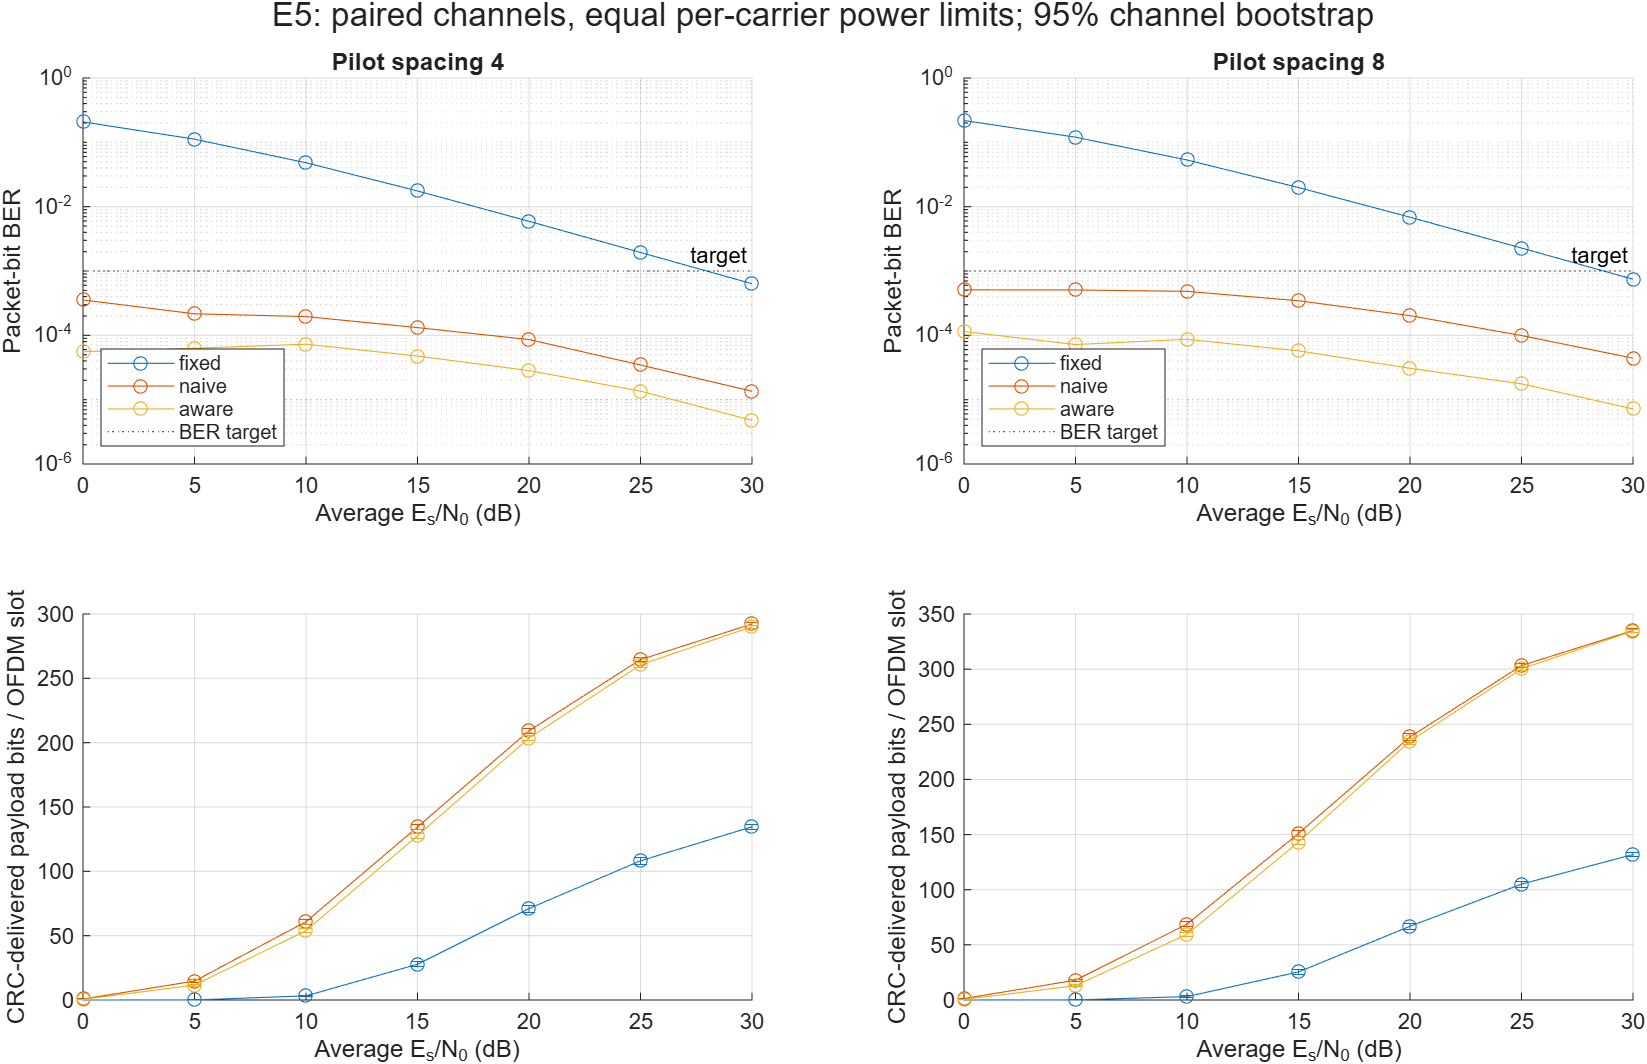
\includegraphics[width=0.92\linewidth]{figures/E5_adaptive.png}
\caption{Adaptive loading over 2400 random channels per point. Top: packet
bit error rate; both adaptive policies stay below the $10^{-3}$ target while
fixed QPSK does not. Bottom: delivered payload per OFDM slot. At 15\,dB,
fixed QPSK delivered 18\% of packets, naive 93\% and aware 98\%.}
\end{figure}

Adaptive loading over real sound needs a feedback path from receiver to
transmitter and is not yet implemented in the acoustic link.

%=====================================================================
\section{What the live experiments show}
%=====================================================================

\begin{figure}[h]
\centering

\includegraphics[width=0.95\linewidth]{docs/img/live_results.png}
\caption{Left to right: transmitted picture; one MacBook to itself (64/64);
phone to MacBook without coding (0/64); phone to MacBook with coding
(63/64). Gray columns are packets rejected by the CRC.}
\end{figure}

\subsection{One device: a near-ideal channel}
Speaker and microphone a few centimetres apart in the same case gave a
median carrier SNR of 30\,dB, EVM $-24\,$dB and only $-28\,$dB of energy
outside the prefix. At 30\,dB, $\Q(\sqrt{1000})$ is astronomically small, so
all 64 packets arrived with zero bit errors at 2045\,bit/s.

\subsection{Phone to laptop without coding}
SNR about 15\,dB and EVM about $-8\,$dB put the raw bit error rate near
$1.2\%$. From the packet formula, $(1-0.012)^{576}\approx0.1\%$: as observed,
no packet passed. The receiver itself was working; the bits were simply not
quite clean enough for an all-or-nothing packet.

\subsection{Phone to laptop with coding}
Same phone, same room. The decoder overruled a median of 19 of the 1164
coded bits per packet ($\approx1.6\%$) and 63 of 64 packets passed. The one
failure needed about 170 corrections (15\%), far more than the code can
handle and far more than the channel's typical error rate, which points to a
brief disturbance during that packet.

\begin{figure}[h]
\centering
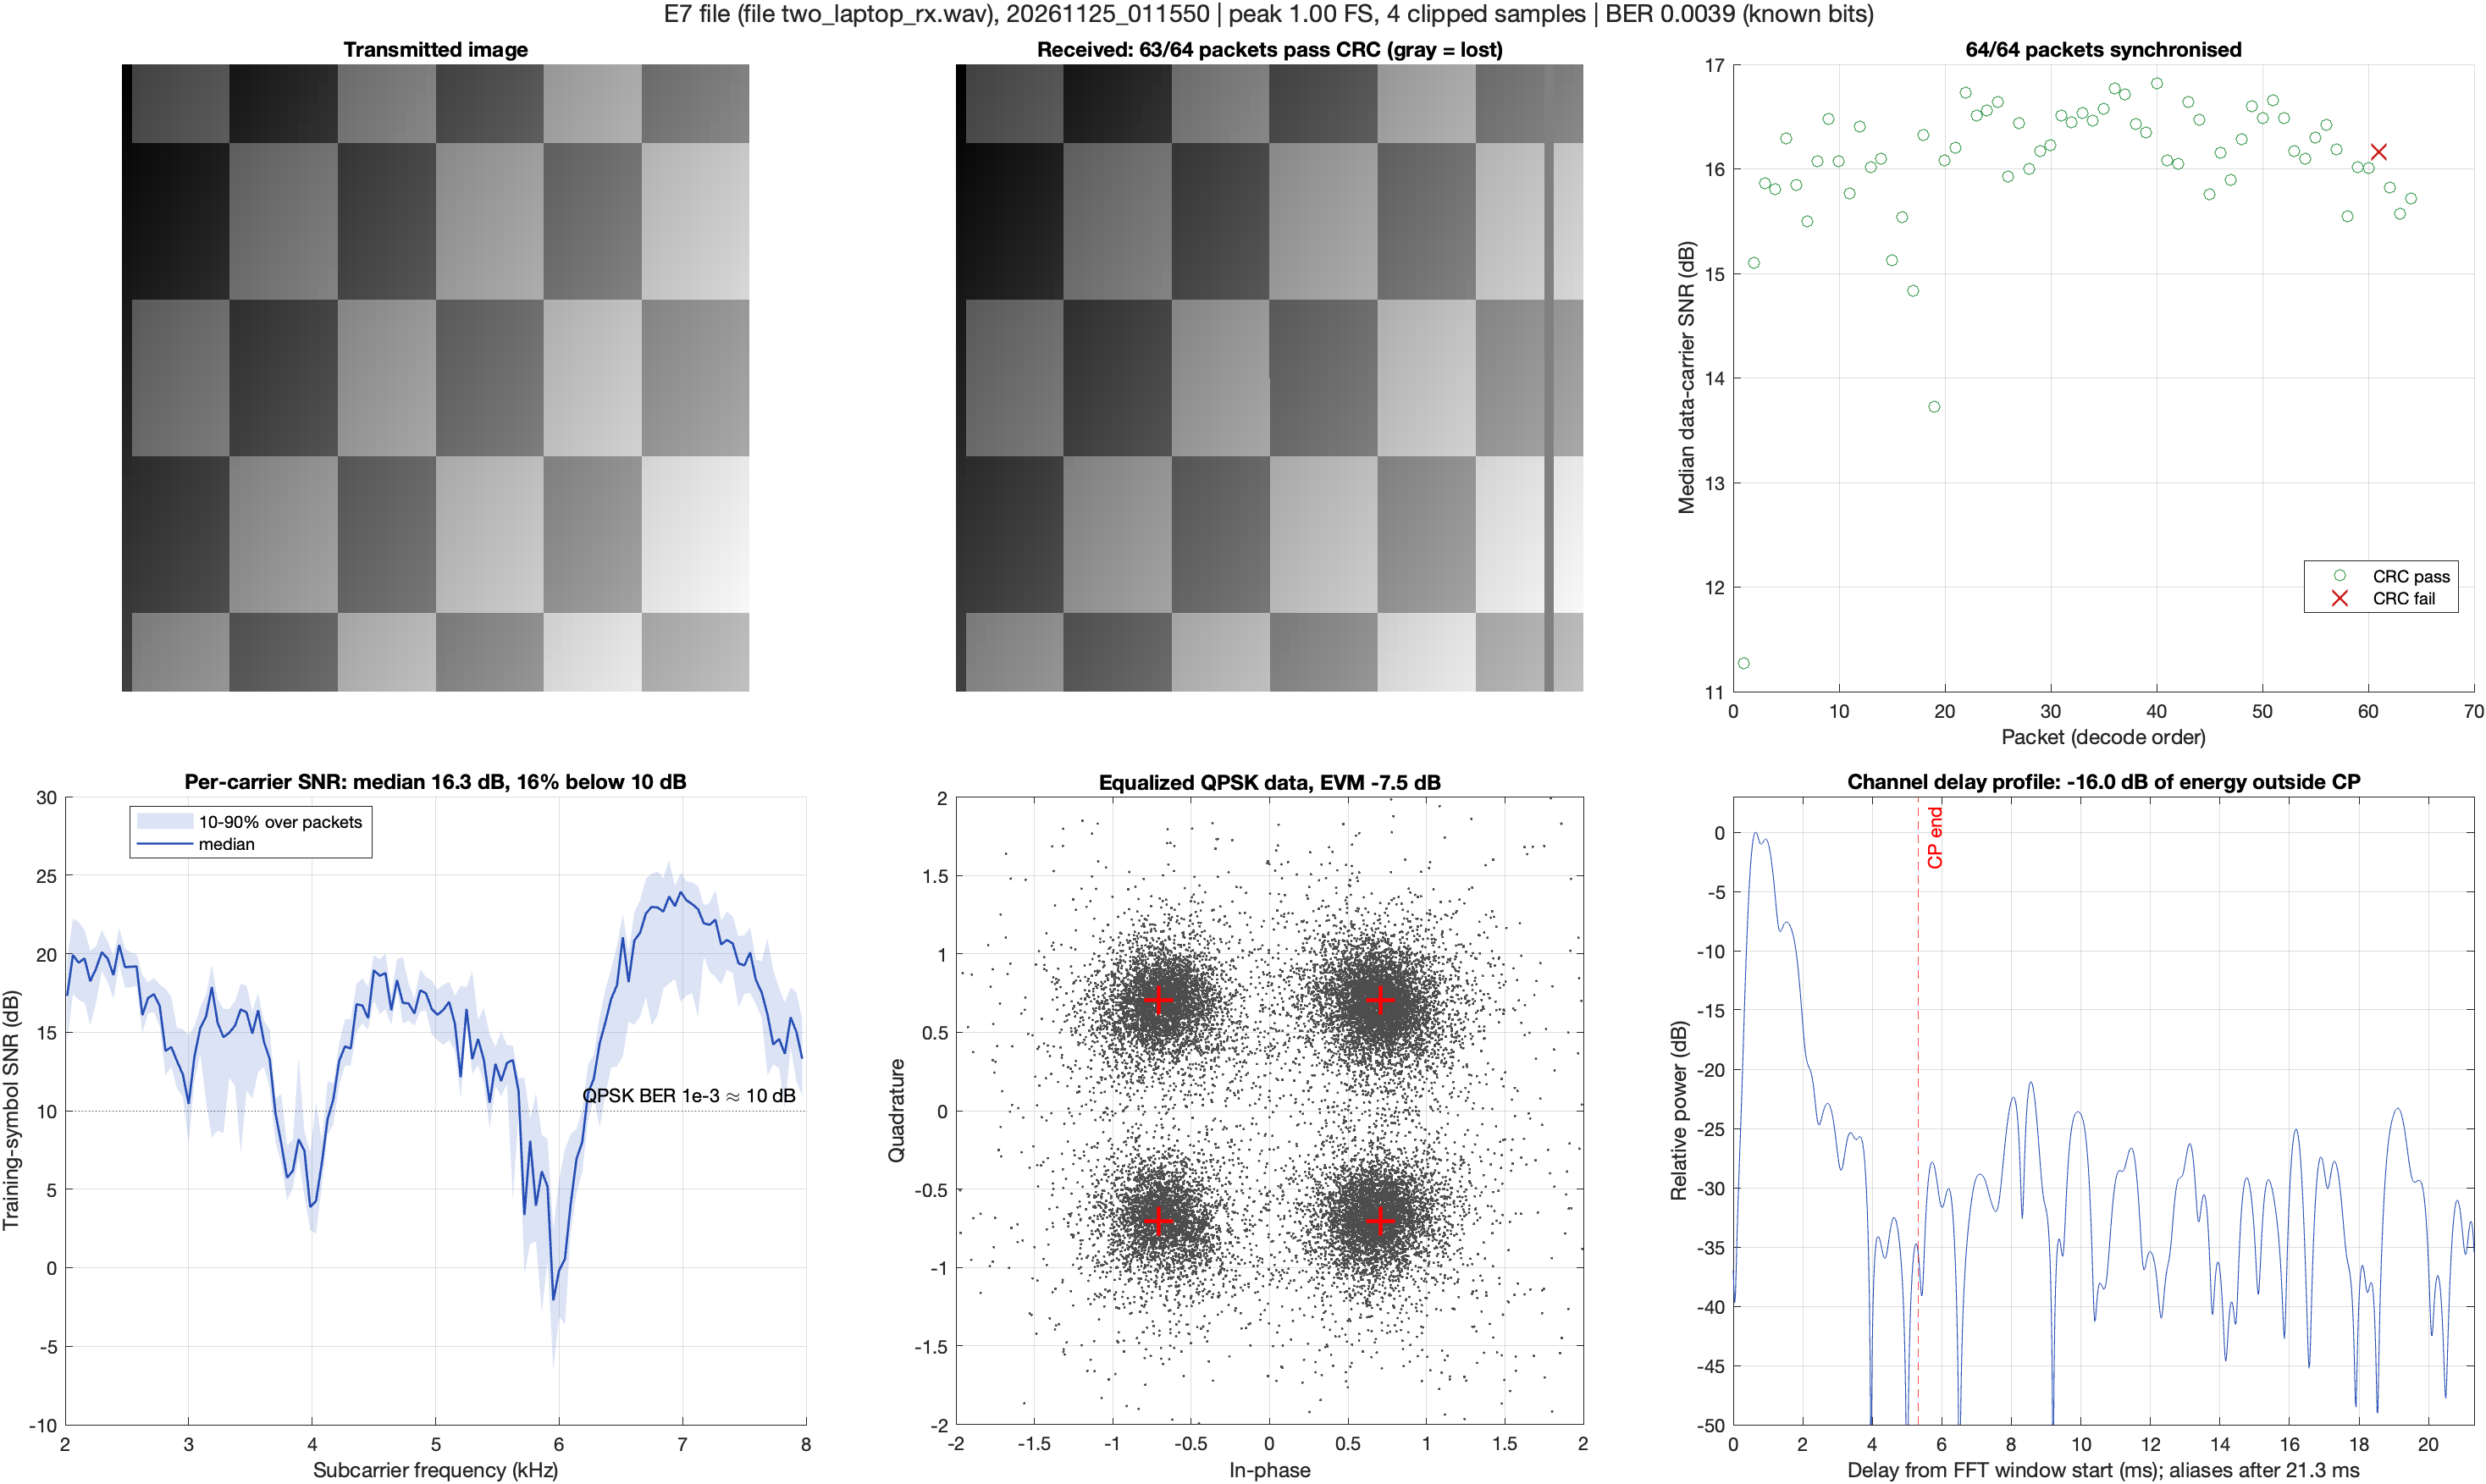
\includegraphics[width=0.95\linewidth]{figures/E7_speaker_file_fec_20261125_011550.png}
\caption{Diagnostics of the coded phone run. Top: sent and received picture,
SNR of each packet (red cross: the one CRC failure). Bottom: SNR per
subcarrier with notches near 4 and 6.5\,kHz, the equalised QPSK
constellation, and the channel delay profile.}
\end{figure}

\subsection{The Windows laptop: when the LTI model breaks}
\label{sec:windows}
Played from a Windows laptop, the signal failed even though, in the
2--8\,kHz band, it was 37\,dB above the room noise. Lowering the volume by
20\,dB left the receiver's SNR unchanged (about 10\,dB), and the EVM was far
worse than that SNR. Additive noise would behave the opposite way. The
recordings also showed the level creeping up during playback. All of this
points to the laptop's audio processing (automatic loudness, dynamic range
compression, ``enhancements''): a nonlinear, time-varying system that
violates \eqref{eq:lti}. Its errors scale with the signal, so they cannot be
escaped by turning the volume up or down, and a training estimate taken at
the start of a packet goes stale by its end.

\subsection{Rooms and distance}
The stress test sends the real waveform through synthetic rooms. With
coding, a desk-like channel (DRR $+12\,$dB, $-16\,$dB outside the prefix)
passes everything; a 1-metre room ($-9\,$dB outside) passes 80--97\%; a
2-metre room ($-4\,$dB outside) passes nothing at any SNR. This is the
interference cap of Section~\ref{sec:cp} in action: beyond a certain
distance the limit is the prefix length, not the noise.

\begin{figure}[h]
\centering
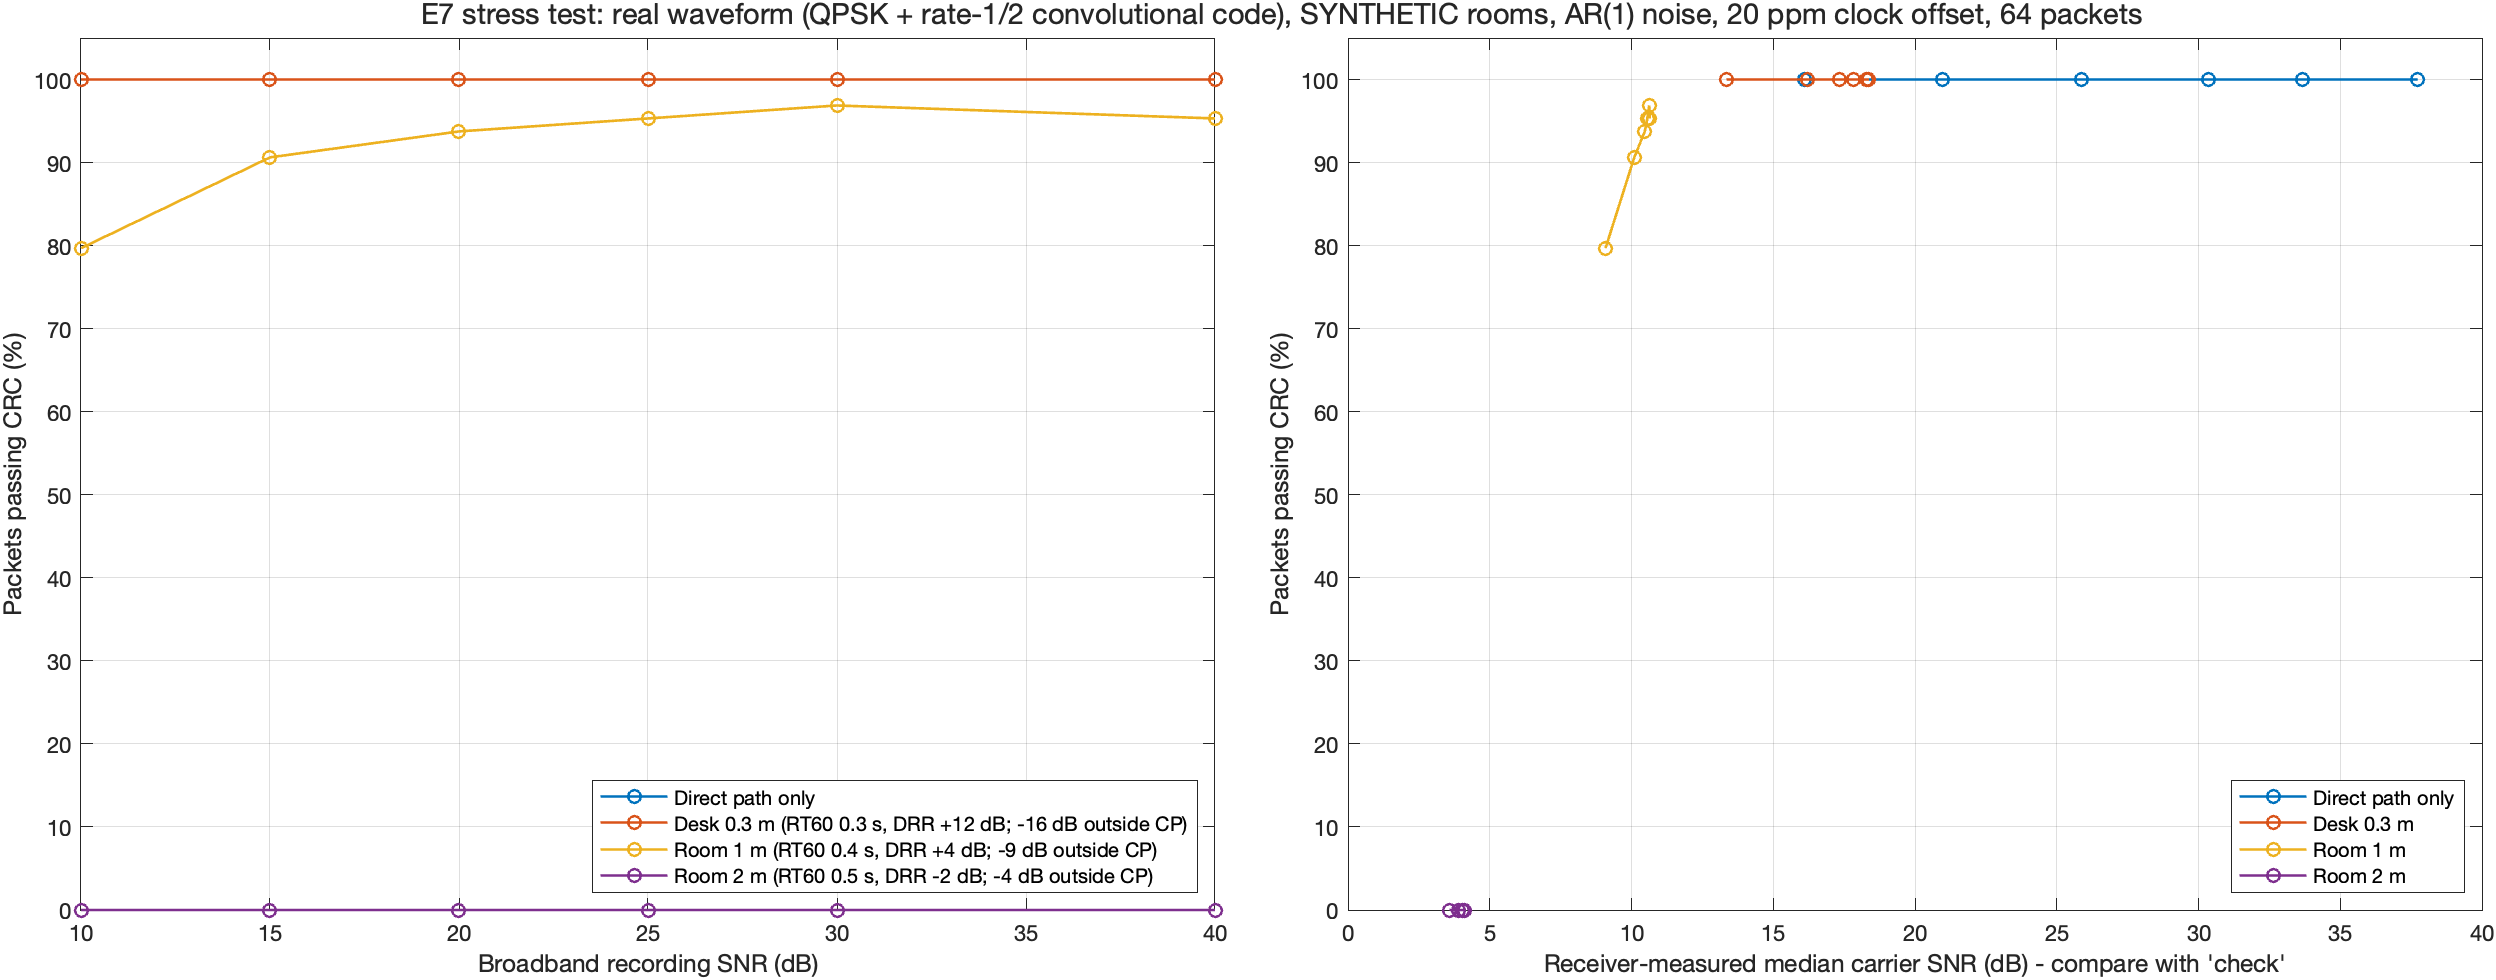
\includegraphics[width=0.95\linewidth]{figures/E7_speaker_stress_fec.png}
\caption{Coded stress test: packets passing against recording SNR (left) and
against the receiver's measured SNR (right) for four synthetic rooms.}
\end{figure}

%=====================================================================
\section{Limits and natural extensions}
%=====================================================================
\begin{itemize}
\item \textbf{Longer echoes.} A longer cyclic prefix (or a longer FFT) would
extend the range into reverberant rooms, at a cost in rate.
\item \textbf{Channel-aware transmission.} In simulation, adaptive loading
delivered several times the throughput of fixed QPSK at mid SNR (about 134
against 28 payload bits per slot at 15\,dB). Doing this acoustically needs
a short feedback message from receiver to transmitter.
\item \textbf{Stronger codes.} Longer packets with LDPC or turbo codes would
approach capacity more closely than the $K=7$ convolutional code.
\item \textbf{Tracking within a packet.} Updating $\hat H_k$ from decided
data (decision-directed estimation) would help with slowly varying channels
and with gentle automatic gain control.
\item \textbf{General transfer.} The receiver currently knows the picture
size; a header describing the payload would allow arbitrary files.
\end{itemize}

\appendix
%=====================================================================
\section{Parameters used in the code}
%=====================================================================
\begin{center}
\begin{tabular}{@{}ll@{}}
\toprule
Sample rate $f_s$ & 48\,kHz \\
FFT size $N$ / subcarrier spacing & 1024 / 46.875\,Hz \\
Cyclic prefix & 256 samples (5.33\,ms) \\
Used bins & 43--170 (2.0--8.0\,kHz), 128 subcarriers \\
Pilots / data subcarriers & every 4th (32) / 96 \\
Modulation & Gray QPSK, $E_s=1$, unitary FFT \\
Training & 2 identical full-band QPSK symbols \\
Preamble & 50\,ms linear chirp, 1$\to$9\,kHz, Hann window \\
Packet & 4 B header + 64 B data + CRC-32 = 576 bits \\
Code (optional) & rate 1/2, $K=7$, generators 133/171 (octal), $d_{\mathrm{free}}=10$ \\
Interleaver & block, $84\times16$ for 1344 coded-bit slots \\
Decoder & soft-decision Viterbi, SNR-weighted LLRs \\
Picture & $64\times64$ 8-bit gray, 64 packets \\
Duration / net rate & 16.0\,s, 2045\,bit/s (uncoded); 22.9\,s, $\approx$1430\,bit/s (coded) \\
\bottomrule
\end{tabular}
\end{center}

\section{Notation}
\label{app:notation}
\begin{center}
\begin{tabular}{@{}ll@{}}
\toprule
$x[n],\,y[n]$ & transmitted and received samples \\
$h[\ell],\,H_k$ & channel impulse response and its value on bin $k$ \\
$X_k,\,Y_k,\,W_k$ & transmitted symbol, received value, noise on bin $k$ \\
$\hat H_k,\,\hat X_k$ & channel estimate, equalised symbol \\
$E_s,\,\sigma^2,\,\gamma$ & symbol energy, noise variance, SNR $=E_s/\sigma^2$ \\
$N,\,N_{\mathrm{cp}}$ & FFT length, cyclic-prefix length \\
$\Q(\cdot)$ & Gaussian tail probability \\
$\bm R,\,\bm C_e$ & channel correlation, estimation-error covariance \\
$\varepsilon$ & relative sample-clock offset \\
LLR & log-likelihood ratio, positive favours bit 0 \\
\bottomrule
\end{tabular}
\end{center}

\section{Where each idea lives in the code}
\begin{center}
\begin{tabular}{@{}ll@{}}
\toprule
Idea & File \\
\midrule
IFFT/FFT, CP, Hermitian mirror & \texttt{ofdm/ofdm\_modulate.m}, \texttt{ofdm\_demodulate.m} \\
QPSK mapping and decisions & \texttt{ofdm/modulate\_bits.m}, \texttt{demap\_symbols.m} \\
Packet and CRC & \texttt{ofdm/make\_packet.m}, \texttt{crc32\_bytes.m} \\
Frame building & \texttt{audio/make\_audio\_frame.m} \\
Chirp and matched filter & \texttt{audio/make\_chirp.m}, \texttt{find\_preamble.m} \\
Estimation, equalisation, LLRs & \texttt{audio/decode\_audio\_frame.m} \\
Pilot phase tracking & \texttt{audio/correct\_pilot\_phase.m} \\
Convolutional code & \texttt{ofdm/fec\_encode.m}, \texttt{fec\_decode.m}, \texttt{fec\_interleaver.m} \\
L-MMSE weights & \texttt{ofdm/estimator\_weights.m} \\
Adaptive loading & \texttt{ofdm/select\_loading.m} \\
Synthetic rooms & \texttt{audio/synthetic\_room.m} \\
\bottomrule
\end{tabular}
\end{center}

\end{document}
